\documentclass[9pt,twocolumn]{paper-template}
% Use the lineno option to display guide line numbers if required.
\usepackage{lipsum}
\usepackage{tabularx} % in the preamble
\usepackage{subcaption}
\usepackage{multirow}
\templatetype{twocolumn} % Choose template 
% {pnasresearcharticle} = Template for a two-column research article
% {pnasmathematics} %= Template for a one-column mathematics article
% {pnasinvited} %= Template for a PNAS invited submission

\title{A Review on Interactive Adaptive Processes Which Underline Short-Term Motor Learning}

% Use letters for affiliations, numbers to show equal authorship (if applicable) and to indicate the corresponding author
\author[a]{MohammadAmin Alamalhoda}
\author[a]{Arsalan Firoozi} 
\author[a]{Mohammad khorshidi}
\affil[a]{Student, EE Department, Sharif University of Technology}

% Please add here a significance statement to explain the relevance of your work
\significancestatement{Multiple models have tried to simulate the motor skill acquisition but most of them fail in producing some of the features of motor skill learning. Here a model is introduced where demonstrate that within a timescale of minutes, two distinct fast-acting processes drive motor adaptation. One process responds weakly to error but retains information well, whereas the other responds strongly but has poor retention. This two-state learning system makes the surprising prediction of spontaneous recovery (or adaptation rebound) if error feedback is clamped at zero following an adaptation-extinction training episode.}

% Please include corresponding author, author contribution and author declaration information
\authorcontributions{Author contributions}
\equalauthors{\textsuperscript{1}All contributed equally to this work}

% Keywords are not mandatory, but authors are strongly encouraged to provide them. If provided, please include two to five keywords, separated by the pipe symbol, e.g:
\keywords{Motor learning } 

\begin{abstract}
Abstract
\end{abstract}

\dates{This manuscript was compiled on \today}

\begin{document}

\maketitle
\thispagestyle{firststyle}
\ifthenelse{\boolean{shortarticle}}{\ifthenelse{\boolean{singlecolumn}}{\abscontentformatted}{\abscontent}}{}

% If your first paragraph (i.e. with the \dropcap) contains a list environment (quote, quotation, theorem, definition, enumerate, itemize...), the line after the list may have some extra indentation. If this is the case, add \parshape=0 to the end of the list environment.
\dropcap{N}ull
\\
\section*{Results}


\textbf{Motor Adaptation Experiments That Show Savings}
Figure \ref{fig:saving} shows simulations of the experimental paradigm that shows savings in eye saccade adaptation. The progress of motor output in learn-unlearn-relearn paradigms with three different models is simulated. Models are (1) a single-state, single time-constant model, (2) a two-state, gain- specific model, and (3) a two-state, gain-independent, multi- rate model. All of these models give motor output as a function of current motor state and the error of last trial. The learning rules for these models are:

\begin{eqnarray*}
& (1)\;Single\;State:\\
& x(n+1) = Ax(n)+Be(n)
\end{eqnarray*}

\begin{eqnarray*}
& (1)\;Gain\;Specific:\\
&x1(n+1) = min(0,[Ax_1(n)+Be(n)])\\
&x2(n+1) = max(0,[Ax_2(n)+Be(n)])\\
&x = x_1+x_2
\end{eqnarray*}


\begin{eqnarray*}
& (1)\;Multi\;Rate:\\
& x1(n+1) = A_fx_1(n) + B_fe(n)\\
& x2(n+1) = A_sx_2(n) + B_se(n)\\
&x = x_1+x_2
\end{eqnarray*}

All of these models have error term ($e(n)$) because there is a difference between the motor output $x(n)$ and the state of the environment $f(n)$, so: $e(n) = f (n) - x(n)$.\\
As can be seen in the results of the simulations, single-state model can't reproduce saving, while both of the gain-specific model proposed by Kojima et al. and multi-rate model proposed by Shadmehr et al. can produce saving. Also, both of these models show decay in the amount of saving when null trials are inserted before the learning block which makes sense based on our intuition of the motor control processes. Because the internal states are different, both systems’ responses to the learning stimulus are altered. Relearning is faster than initial learning in the gain-specific model because both the up and down states can contribute to relearning whereas only the up state contributes to initial learning. In the case of the multi-rate model, relearning is faster than initial learning because when relearning starts, the
slow state is already biased towards relearning, making relearning more dependent on the fast state compared to initial learning.\\



\begin{figure*}[h!]
  \centering
    \includegraphics[width=\linewidth]{figures/figure1/Fig}
  \caption{\textbf{Simulations of Motor Adaptation Experiments That Show Savings}\\
  (A) shows the model simulations of the experiment paradigm (Disturbance plot) which is plotted in black. (B) shows a direct comparison of simulated performance in the initial learning and relearning blocks.  (C) shows the amount of savings found in simulation, as a function of the number of washout trials. The amount of savings is measured as the percent improvement in performance on the 30th trial in the relearning block compared to the 30th trial in the initial learning block. 
}
  \label{fig:saving}
\end{figure*}


\textbf{Anterograde Interference Simulation}
It’s been reported that an initial motor adaptation has faster time constant in comparison with subsequent adaptation for the oppositely directed stimulus. [\cite{Bizzi}, \cite{shadmehr_jn}, \cite{Wolpert}] We’ve tested the multi-rate model under different stimuli and the result clearly shows we have faster time constant for the initial adaptation. 
The first stimulus is Anterograde interference which consists of a number of trials (In this case: 30, 60 and 120) as adaptation and 50 trials as deadaptation (Figure \ref{fig:Anterograde_Interference_Simulation} A). In Figure \ref{fig:Anterograde_Interference_Simulation} B, the raw response of multi-rate model is shown; Also, in Figure \ref{fig:Anterograde_Interference_Simulation} D and F, you can see the response of Gain-specific model and Single State model. By comparing the time constants of each model (Figure \ref{fig:Anterograde_Interference_Simulation} C, E, and G), results show that only multi-rate model has higher time constant in the initial adaptation; Single state model shows no change of time constant and Gain specific model shows faster time constant for the secondary adaptation. Since we have a bias against the deadaptation, it is expected to have slower time constant in the secondary adaptation in multi-rate model.\\



\textbf{Deadaptation Simulation }
The second stimulus is Deadaptation Simulation which consists of a number of trials (In this case: 30, 60 and 120) as adaptation and then trials back to base line (Figure \ref{fig:Deadaptation_Simulation} A). There are studies reporting that the rate of deadaptation is faster than the rate of initial adaptation [\cite{Wolpert}, \cite{shadmehr_jnp}]. Results show that the multi rate model and the gain specific model show faster rate of deadaptation while the single state model shows no changes in the rate (Figure \ref{fig:Deadaptation_Simulation} C, E, and G). Also it can be inferred that by increasing the number of adaptation trials, the rate of deadaptation decreases.\\


\textbf{Down-Scaling Simulation}
It is reported that the time constant of adapting to a lower level of previously learnt adaptation is faster than deadaptation to baseline. In Figure \ref{fig:Down_Scaling_Simulation} we showed that the multi rate model can explain this effect while the single state model and the gain specific model cannot. It can be seen that the Gain specific model shows somehow inverse effect.





\textbf{Robustness of spontaneous rebound in the multi-rate model}\\
A key feature of the multi-rate model is its ability to predict the spontaneous recovery. Figure \ref{fig:multi_rate_recovery} only shows spontaneous recovery for
specific sets of model parameters, however spontaneous recovery is a general feature of this
model over a very wide space of model parameters. Because an analytical approach to
demonstrating this property is difficult, we performed a large set of simulations in which the
model parameters where systematically varied (by as much as a factor of 10). In these simulations the fractional spontaneous
recovery (max rebound/max initial learning) was assessed following asymptotic learning and
unlearning to baseline. The results of these simulations are shown in Figure \ref{fig:mutli_rate_params}. There are four
parameters in the multi-rate model and each panel below displays the amount of
spontaneous recovery when two of these parameters are systemically varied. There are six
panels because there are six different two-parameter combinations. Note that in all cases
more than 80\% of the parameter space shown displays a spontaneous recovery of greater
than 20\%, where the amount of spontaneous recovery refers to the ratio of the maximum
recovery in the error clamp phase to the asymptotic amount of learning during the initial
learning phase. These simulations show that spontaneous recovery is a robust feature of
the multi-rate model in this experimental paradigm, and that the finding of spontaneous
recovery does not depend upon a narrow choice of parameter values.

\begin{figure}[h!]
  \centering
     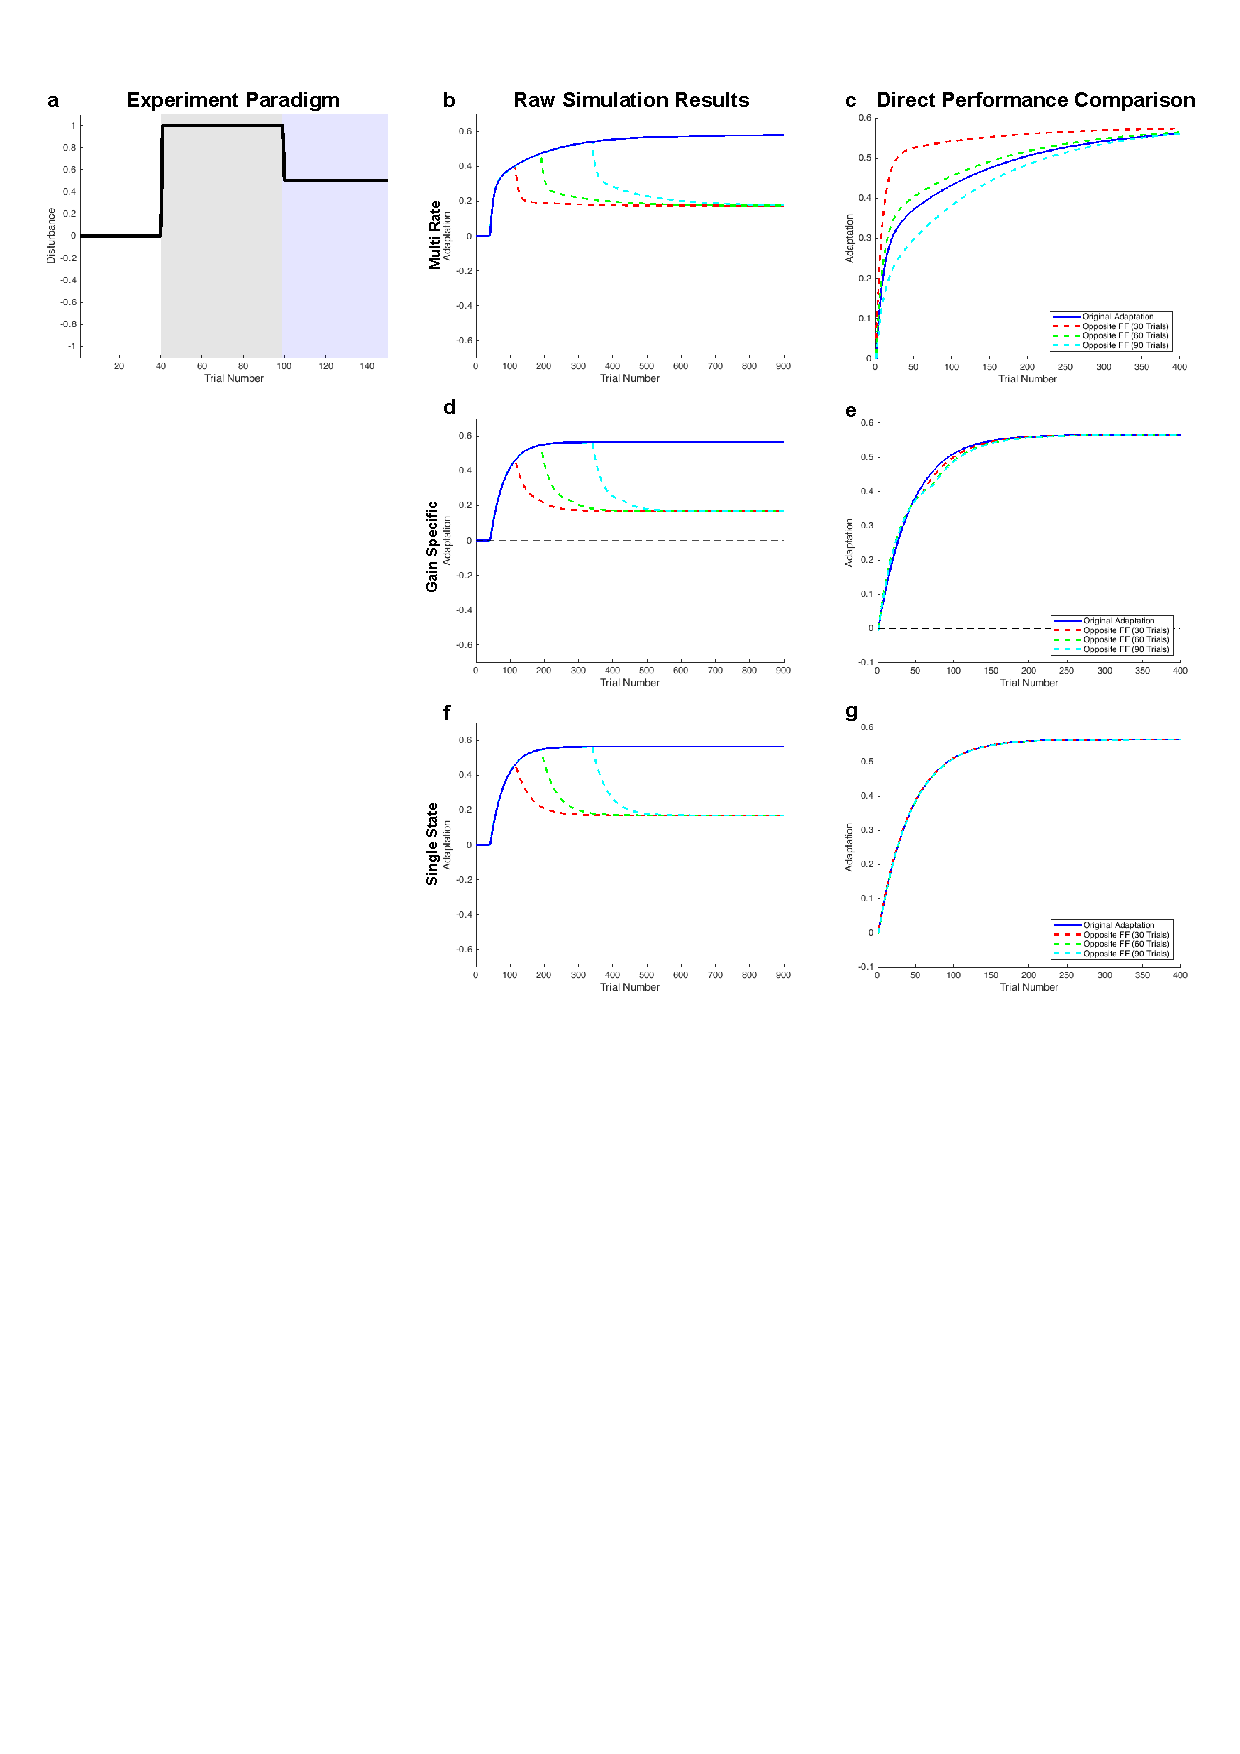
\includegraphics[width=\linewidth]{figures/Fig6}
  \caption{\textbf{Anterograde Interference Simulation}\\(A)  Experiment Paradigm. (B, D, F) Raw simulation results of Multi Rate model, Gain Specific model, and Single State model. Blue: initial adaptation. Red, Green, Cyan: secondary adaptation after 30, 60, 120 initial adaptation trials. (C, E, G) Direct performance comparison of Multi Rate model, Gain Specific model, and Single State model. In this column learning curves are shifted and scaled so that the desired performance is one. In this paradigm only multi-rate model has higher time constant in the initial adaptation comparing to the time constant of deadaptation; Single state model shows no change of time constant and Gain specific model shows faster time constant for the secondary adaptation. Since we have a bias against the deadaptation, it is expected to have slower time constant in the secondary adaptation in multi-rate model. And the results show that in multi rate model we get slower time constant by increasing the number of adaptation trials. 
}
  \label{fig:Anterograde_Interference_Simulation}
\end{figure}


\begin{figure}[h!]
  \centering
     \includegraphics[width=\linewidth]{figures/Fig7}
  \caption{\textbf{Deadaptation Simulation}\\ (A)  Experiment Paradigm. (B, D, F) Raw simulation results of Multi Rate model, Gain Specific model, and Single State model. Blue: initial adaptation. Red, Green, Cyan: secondary adaptation after 30, 60, 120 initial adaptation trials. (C, E, G) Direct performance comparison of Multi Rate model, Gain Specific model, and Single State model. In this column learning curves are shifted and scaled so that the desired performance is one. In this paradigm the multi rate model and the gain specific model show faster rate of deadaptation while the single state model shows no changes in the rate. Also it can be inferred that by increasing the number of adaptation trials, the rate of deadaptation decreases. 
}
  \label{fig:Deadaptation_Simulation}
\end{figure}


\begin{figure}[h!]
  \centering
     \includegraphics[width=\linewidth]{figures/Fig8}
  \caption{\textbf{Down-Scaling Simulation}\\ (A)  Experiment Paradigm. (B, D, F) Raw simulation results of Multi Rate model, Gain Specific model, and Single State model. Blue: initial adaptation. Red, Green, Cyan: secondary adaptation after 30, 60, 120 initial adaptation trials. (C, E, G) Direct performance comparison of Multi Rate model, Gain Specific model, and Single State model. In this column learning curves are shifted and scaled so that the desired performance is one. In this paradigm the multi rate model shows the effect of having faster time constant of adapting to a lower level of previously learnt adaptation than deadaptation to baseline. The Gain specific model shows somehow inverse effect.
}
  \label{fig:Down_Scaling_Simulation}
\end{figure}











\textbf{Memory of errors}\\

As Shadmeher et al. stated in their paper (\cite{mem_error}), The brain learns more from the error when it is consistent in time. This is implemented in their model by $\eta$ which is error-sensitivity parameter. They assumed the action $u(n)$ to be zero.So, the model becomes:

\begin{eqnarray*}
& e^{(n)} = x^{(n)}-\hat{x}^{(n)}\\
& \hat{x}_{n+1} = \alpha \hat{x}_n + \eta_ne_n
\end{eqnarray*}
where  each basis element $g_i$ has a preferred error $e^\smallsmile$ and:
\begin{eqnarray*}
& \eta(e^{(n)}) = \sum_i^N \omega_ig_i(e^{(n)})\\
&g_i(e^{(n)}) = e^{\frac{-(e^{(n)}-{e^\smallsmile}_i)^2}{2\sigma^2}}
\end{eqnarray*}

On trial $n-1$ the motor command $u(n-1)$ produces an error $e(n-1)$ , the nervous system learns from this error and produces motor command $u (n)$ on the subsequent trial, resulting in $e(n)$ . In a slowly switching environment (Figure \ref{fig:herzfeld} A), $e(n)$ has the same sign as $e(n-1)$ . In this case, error-sensitivity should increase around $e(n-1)$ On the other hand, in a rapidly switching environment (\ref{fig:herzfeld} A), $e(n)$ has a different sign than $e(n-1)$ . In this case, error-sensitivity should decrease:

\begin{eqnarray*}
& \omega^{(n+1)} =omega^{(n)}+\beta sign(e^{(n-1)}e^{(n)}) \frac{g(e^{(n-1)})}{g^T(e^{(n-1)})g(e^{(n-1)})}\\
&g_i(e^{(n)}) = exp(\frac{-(e^{(n)}-{e^\smallsmile}_i)^2}{2\sigma^2})
\end{eqnarray*}

We have simulated this model and the results are shown in Figure \ref{fig:herzfeld}. Also the relation between the speed of changes in environment with error-sensivity is plotted shown in Figure \ref{fig:herzfeld} B. 

\section*{Material and Method}
We used specific learning rates and formulas below for obtaining the output of the models stated in the text.

\begin{eqnarray*}
& perturbation\;trials : e(n)=f(n)-x(n)\\
& error-clamp trials : e(n) = 0\\
& e(n) = error\;on\;trial\;n\\
& x(n) = adapted\;motor\;output\;on\;trial\;n\\
& f(n) = disturbance\;on\;trial\;n
\end{eqnarray*}

For all of the figures, parameters of the single-state and gain-specific models are set as $A=0.99$, $B=0.013$ and for the multi-rate are set as $A_f = 0.92$, $A_s = 0.996$, $B_f = 0.03$, and $B_s = 0.004$. Also, as shown in Figure \ref{fig:mutli_rate_params}, the qualitative results that are described in the text do not depend on these particular parameter values; they hold as long as all parameters are positive, and $B_f$ is several-fold larger than $B_s$, and $A_s$ is several times closer to one than $A_f$.

The number of washout trials was varied from 0 to 300, and the percent savings was computed for each simulation as the performance improvement on trial 30 of the relearning block versus trial 30 of the initial learning block. All of the simulations were done using Matlab.

\begin{figure}[h!]
  \centering
  \begin{subfigure}[b]{0.32\linewidth}
    \includegraphics[width=\linewidth]{figures/figure5/Af_AS}
  \end{subfigure}
  \begin{subfigure}[b]{0.32\linewidth}
    \includegraphics[width=\linewidth]{figures/figure5/Af_Bf}
  \end{subfigure}
   \begin{subfigure}[b]{0.32\linewidth}
    \includegraphics[width=\linewidth]{figures/figure5/Af_Bs}
  \end{subfigure}
    \begin{subfigure}[b]{0.32\linewidth}
    \includegraphics[width=\linewidth]{figures/figure5/As_Bf}
  \end{subfigure}
  \begin{subfigure}[b]{0.32\linewidth}
    \includegraphics[width=\linewidth]{figures/figure5/As_Bs}
  \end{subfigure}
   \begin{subfigure}[b]{0.32\linewidth}
    \includegraphics[width=\linewidth]{figures/figure5/Bf_Bs}
  \end{subfigure}
  \caption{\textbf{Simulation of the effects of different learning rates and forgetting factors on the amount of the spontaneous rebound predicted by the multi-rate model}\\
  All of the plots show value of the spontaneous rebound vs different parameters of the multi-rate model. default value of the parameters is: $A_f=0.92$, $A_s=0.996$, $B_f=0.03$, and $B_s=0.004$. The amount of the spontaneous rebound is measured as ratio of maximum recovery in the error-clamp phase to the asymptotic amount of learning during the initial learning phase. 
}
  \label{fig:mutli_rate_params}
\end{figure}



\begin{figure}[h!]
  \centering
    \includegraphics[width=\linewidth]{figures/figure4/Fig}
  \caption{\textbf{Herzfeld Theoretical model}\\
  {(A)} presents model performance for slow, medium, and rapidly switching environments (gray line represents $\hat{x}^{(n)}$. {(B)} shows the error-sensivity value over the trials for different values of Z. Z is the speed of switching of the environment. Bigger error-sensivity values lead to less learning from the error, so model learns more from slow switching environments in comparison with rapidly switching environments.
}
  \label{fig:herzfeld}
\end{figure}















\newpage

\acknow{We highly appreciate ... }

\showacknow{} % Display the acknowledgments section

\section*{References}
% Bibliography
\bibliography{References}

\bigskip
\begin{center}
All codes are available at \href{https://github.com/MohammadAminAlamalhoda/Motor-Learning}{this link}.
\end{center}
\end{document}